\documentclass[11pt,a4paper]{article}
\usepackage[latin1]{inputenc}
\usepackage{amsmath}
\usepackage{amsfonts}
\usepackage{amssymb}
\usepackage{graphicx}
\author{Jordan Murray}
\title{EECS305 Lab5}
\begin{document}
\begin{center}
\fontsize{24}{12}\selectfont
\textbf{Experiment 5: Lead-Lag Control of a DC Servo Motor}
\end{center}
\section{OBJECTIVES}

\begin{enumerate}
\item Identify the parameters of a system using frequency domain observations.

\item Understand the impact of feedback gain on frequency domain behavior.

\item Determine the phase and gain margin from bode plots.

\end{enumerate}


\section{BASIC KNOWLEDGE}
In this experiment, we introduce mathematical models for a DC servomechanism.

\subsection{Background information on DC servo motor system}

A block diagram for a typical servomechanism is shown in Fig. ~\ref{fig:servoblock}.  The action of the servomechanism is to track a desired position (or speed) despite the 
presence of disturbance inputs to the process and despite errors in the 
sensor data.

\begin{figure}[here]
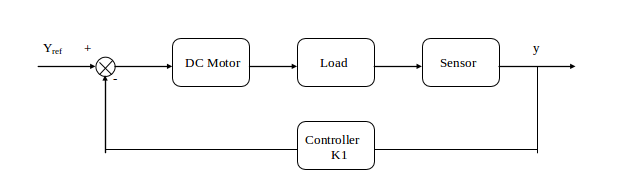
\includegraphics[width=\textwidth]{imglab/servoblockdiagram.png}
\caption{Servomechanism block diagram}
\label{fig:servoblock}
\end{figure}

\subsubsection{Model Development}
\begin{figure}[here]
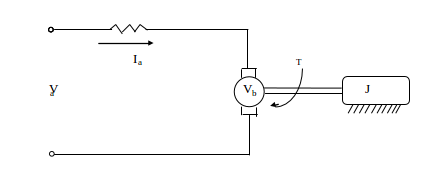
\includegraphics[width=\textwidth]{imglab/servoschemdiagram.png}
\caption{schematic diagram of the DC servo motor}
\label{fig:servoschem}
\end{figure}

We begin by developing a simplified linear model of an armature controlled DC servo motor and load. Fig. ~\ref{fig:servoschem} shows the schematic diagram of the motor and load.

Neglecting the inductance of the armature circuit, the armature voltage V$_{a}$ produces a current I$_{a}$ as given by:

\begin{equation} \label{eq:1}
I_{a} = \frac{V_{a}-V_{b}}{R_{a}}
\end{equation}

Here V$_{b}$ denotes the back emf of the motor and R$_{a}$ is the armature resistance.

The motor torque T is proportional to I$_{a}$:

\begin{equation} \label{eq:2}
T = K_{T}I_{a}
\end{equation}

But from Newton's law, assuming an inertia load:

\begin{equation} \label{eq:3}
T = J\ddot{\theta}
\end{equation}

combining equations \ref{eq:1}, \ref{eq:2}, and \ref{eq:3} we obtain:

\begin{equation} \label{eq:4}
K_{T}\left[\frac{V_{a}-V_{b}}{R_{a}}\right] = J\ddot{\theta}
\end{equation} 

Using the relationship V$_{b}$ = K$_{b}\dot{\theta}$ and, letting V$_{a}$ = U (input signal), we have:

\begin{equation} \label{eq:5}
\frac{K_{T}}{R_{a}}\left[U-K_{b}\dot{\theta}\right] = J\ddot{\theta}
\end{equation}

\begin{equation} \label{eq:6}
\frac{JR_{a}}{K_{T}}\ddot{\theta}+ K_{b}\dot{\theta} = U
\end{equation}

\begin{equation} \label{eq:7}
\ddot{\theta} + \frac{K_{b}K_{T}}{JR_{a}}\dot{\theta} = \frac{K_{T}}{JR_{a}}U
\end{equation}

or letting $\omega$ = $\dot{\theta}$, and 

\begin{equation} \label{eq:8}
\dot{\omega} + \frac{K_{b}K_{T}}{JR_{a}}\omega = \frac{K_{T}}{JR_{a}}U
\end{equation}

Equations \ref{eq:7} and \ref{eq:8} are the differential equations for the DC motor.

Let $\frac{K_{b}K_{T}}{JR_{a}} = \frac{1}{\tau}$, $\frac{K_{T}}{JR_{a}} = \frac{K_{0s}}{\tau}$. Here, $K_{0s}$ is the static gain and $\tau$ is the time constant of the system from input voltage to output speed. From D.E. \ref{eq:7} we can have the following transfer function:

\begin{equation} \label{eq:9}
\frac{\theta(s)}{U(s)} = \frac{K_{0s}}{s(\tau s + 1)}
\end{equation}

And from D.E. \ref{eq:8} we obtain the transfer function of the DC motor from U to $\dot{\theta}=\omega$:

\begin{equation} \label{eq:10}
\frac{\omega (s)}{U(s)} = \frac{K_{0s}}{(\tau s + 1)}
\end{equation}

Considering the measurements of speed and position, the system can be depicted as in Fig. ~\ref{fig:servomeasschem}

\begin{figure}[here]
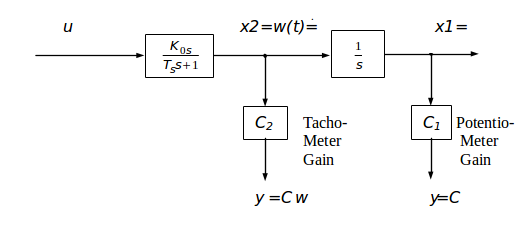
\includegraphics[width=\textwidth]{imglab/servomeasurementschematic.png}
\caption{schematic of the DC motor system with measurements}
\label{fig:servomeasschem}
\end{figure}

Then, the second order D.E. of the DC motor can be rewritten in the state-space format:

$x = A\dot{x} + Bu$
$y = Cx$

where, $x = \left[\begin{matrix}x_{1} \\ x_{2}\end{matrix}\right]$, $u=u$, $y = \left[\begin{matrix}y_{1} \\ y_{2}\end{matrix}\right]$, and
$A = \left[\begin{matrix}0 & 1 \\ 0 & -\frac{1}{\tau}\end{matrix}\right]$, $B=\left[\begin{matrix} 0 \\ \frac{K_{s}}{\tau} \end{matrix}\right]$, $C = \left[\begin{matrix}C_{1} & 0 \\ 0 & C_{2} \end{matrix}\right]$

Further, the input/output transfer function of the DC motor is:

\begin{equation} \label{eq:11}
G(s)=\frac{Y(s)}{U(s)} = \left[ \begin{matrix} G_{1}(s) \\ G_{2}(s) \end{matrix} \right] = \left[ \begin{matrix} \frac{C_{1}K_{0x}}{s(\tau s + 1)} \\ \frac{C_{2}K_{0s}}{\tau s + 1} \end{matrix} \right] = \left[ \begin{matrix} \frac{\left(\frac{C_{1}}{C_{2}}\right)*C_{2}K_{0s}}{s(\tau s + 1)} \\ \frac{C_{2}K_{0s}}{\tau s + 1} \end{matrix} \right]
\end{equation}

Define: $C_{s}=C_{1}/C_{2} and K_{s}=C_{2}K_{0s}$, then

\begin{equation} \label{eq:12}
G(s)=\frac{Y(s)}{U(s)} = \left[ \begin{matrix} G_{1}(s) \\ G_{2}(s) \end{matrix} \right] = \left[ \begin{matrix} \frac{C_{s}K_{s}}{s(\tau s + 1)} \\ \frac{K_{s}}{\tau s + 1} \end{matrix} \right]
\end{equation}

The model has one pole at the origin and one pole on the negative real axis. The problem is to identify parametesr $K_{s}, \tau$ and $C_{s}$. From \ref{eq:12}, the transfer function from input u to output $y_{2}$ is:

\begin{equation} \label{eq:13}
\frac{Y_{2}(s)}{U(s)} = \frac{K_{s}}{\tau s + 1}
\end{equation}

The step response of the first order system is shown in Fig. ~\ref{fig:servostepresp}:

\begin{figure}[here]
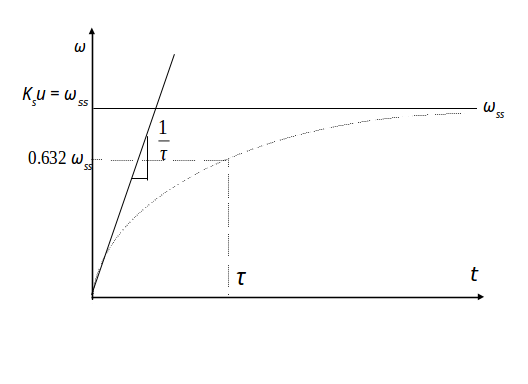
\includegraphics[width=\textwidth]{imglab/servostepresponse.png}
\caption{step response of the DC servo motor}
\label{fig:servostepresp}
\end{figure}

From this diagram, we can determine that the time constant of the motor, $\tau$, is the time it takes $y_{2}$ to reach 63.2\% of its steady state value $y_{2ss}$. We can also obtain the steady-state gain $K_{s} = \frac{y_{2ss}}{U_{ss}}$.

In addition, notice that regarding $C_{s}$ there is a conformity that has to be satisfied:

\begin{equation} \label{eq:14}
C_{s} = \frac{\frac{dy_{1}}{dt}}{y_2}
\end{equation}
This gives the way to identify $C_{s}$.

\subsubsection{Closed Loop Control for a DC servomechanism}
The block diagram of Fig. ~\ref{fig:servoblock} for the servomechanism can be simplified into the block diagram given in Fig. ~\ref{fig:servotfblock}.

\begin{figure}[here]
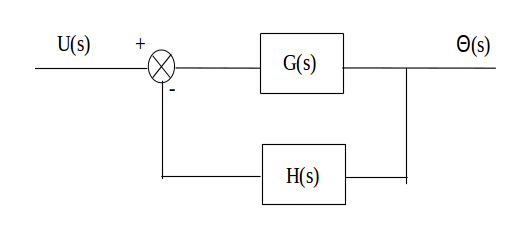
\includegraphics{imglab/servotfblock.png}
\caption{simplified block diagram}
\label{fig:servotfblock}
\end{figure}

This configuration is referred to as a negative feedback closed loop configuration where G(s) is the forward loop transfer function and H(s) is the feedback loop transfer function. The equivalent transfer function between the input r(t) and the output y(t) as shown in Fig. ~\ref{fig:servostepresp} can be represented as the transfer function G'(s) shown in Fig. ~\ref{fig:servocltfblock}.

\begin{figure}[here]
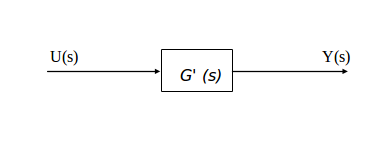
\includegraphics{imglab/servocltfblock.png}
\caption{eqivalent closed-loop transfer function}
\label{fig:servocltfblock}
\end{figure}

\begin{equation} \label{eq:15}
G'(s)=\frac{Y(s)}{U(s)}=\frac{G(s)}{1+G(s)H(s)}
\end{equation}

Considering the servomechanism transfer function:

From Eq. \ref{eq:9}: $G(s)=\frac{C_{s}K_{s}}{s(\tau s + 1)}$,

H(s) = K$_{1}$ (Output feedback controller gain),

\begin{equation} \label{eq:16}
G'(s)=\frac{\frac{C_{s}K_{s}}{\tau}}{s^{2} + \frac{s}{\tau} + \frac{K_{1}K_{s}C_{s}}{\tau}}
\end{equation}

We observe that the transfer function of the closed-loop system, G'(s) is a second order system with one free controller parameter $K_{1}$. Changing the gain $K_{1}$ can be used to alter the transient dynamics of the second order system.


\section{EXPERIMENTAL PROCEDURES}
\subsection{Identify $K_{s}$, $\tau$, $C_{s}$:}
\begin{enumerate}
\item You should have identified these parameters of the DC servo model in a previous lab, but now we will attempt to measure them in a different way.

\item Run \textbf{MATLAB} and open the model \textbf{LabFD\_OLFreqResponse.slx}. It contains an open loop DC servo model fed by a sinusoidal input.

\item Adjust the frequency of the sinusoidal input block over a range sufficient to capture the interesting features of the system's frequency response.  You might try something like the following: begin with frequencies of {.1,.2,.5,1,2,5,10,20,..} until the asymptotic phase values are approached, then try more points as necessary near the cutoff frequency. Measure and record the amplitude and relative (to the input signal) phase of both the \textbf{speed and position} trajectories for each frequency.

\item $K_{s}$ can be determined from the initial value of the speed transfer function. The inverse of $\tau$ can be determined by finding the frequency of the position phase response inflection point. $C_{s}$ can be calculated from the parameters already determined and one of the position transfer function data points. Alternatively, you could  use a curve fitting tool to find the parameters. How do the parameter values obtained compare to those determined from time domain measurements?

\item Compare the step responses of the transfer functions with experimentally determined parameters (both those obtained from time domain measurements and those obtained from frequency domain measurements) to that of the DC servo block. Which set of parameter values result in a better model? Why do you think this is?

\item Make a Bode plot of the transfer function. Superimpose the data points you collected.

\item Determine the gain and phase margins for this transfer function.

\end{enumerate}



\subsection{Frequency Domain Effects of Feedback}
\begin{enumerate}
\item Open the model \textbf{LabFD\_CLFreqResponse.slx}. It contains a closed loop DC servo model with a sinusoidal input and position feedback. The feedback gain has been placed in the forward path.

\item Calculate the closed-loop transfer function of this system with unity gain using your estimated parameter values for the open loop transfer function (you can use the parameters determined in this lab or those determined previously, whichever seem to be more accurate).

\item Make one or more Bode plot(s) showing curves for the closed-loop input-position transfer functions resulting from the following gain constants being used in the forward path on position feedback: {.1, 1, 10, 100, 1000}.  Give an expression for the closed-loop transfer function and the phase and gain margins for each.

\item Repeat the previous step for the input-speed transfer function with speed feedback instead of position feedback.

\end{enumerate}



\section{REPORT}
\begin{enumerate}
\item Plot the transients responses from \ref{ss:transient}. Compare the results of the three situations. Comments are needed to describe the effects of the lead compensator and lag compensator and illustrate why they have those effects.
\item Show the detailed procedure of designing the lead compensator based on the root-locus approach. What parameters did you determine for the servo motor? What values did you calculate for $\zeta$ and $\omega_{n}$? What about the zero and pole locations and the gain for the lead compensator? Were you able to meet the specifications laid out in ~\ref{ss:specs}?
\item Design the lead compensator in a more simple way. Design a lead-lag compensator and show how and why it becomes a lead or lead-lag compensator.
\end{enumerate}
\textbf{Question:} We determined that the time constant of the motor, $\tau$, is the time it takes for $y_{2}$ to reach 63.2\% of its steady state value $y_{2ss}$, why?


\end{document}
